\documentclass[a4paper]{article}
\usepackage[UTF8]{ctex}
\usepackage{geometry}
\usepackage{graphicx}
\usepackage{url}
\usepackage{multirow}
\usepackage{array}
\usepackage{booktabs}
\usepackage{url}
\usepackage{enumitem}
\usepackage{graphicx}
\usepackage{float}
\usepackage{amssymb}
\usepackage{amsmath}
\usepackage{subfig}
\usepackage{longtable}
\usepackage{pifont}
\usepackage{color}

\allowdisplaybreaks

\geometry{a4paper, scale=0.78}

% \begin{figure}[H]
%     \centering
%     \includegraphics[width=.55\textwidth]{E.png}
%     \caption{矩阵与列向量的乘法}
%     \label{fig:my_label_1}
% \end{figure}

% \left\{
% \begin{array}{ll}
%       x+2x+z=2 & \\
%       3x+8y+z=12 & \\
%       4y+z=2
% \end{array}
% \right.

% \begin{enumerate}[itemindent = 1em, itemsep = 0.4pt, parsep=0.5pt, topsep = 0.5pt]

% \end{enumerate}

%\stackrel{a}{\longrightarrow}

%\underbrace{}_{} %下括号

%\tableofcontents %目录,并且目录页不记录页码
% \tableofcontents
% \newpage
% \setcounter{page}{1} %new page
% \clearpage

\title{Conditional Random Field}
\author{Chen Gong}
\date{20 February 2020}

\begin{document}
\maketitle
%\pagestyle{empty}
\tableofcontents
\newpage
%\pagestyle{fancy}
\setcounter{page}{1} %new page
\clearpage
\section{Introduction}
本讲主要介绍的是条件随机场(Conditional Random Field),这个东西在机器学习中,曾经有过较大的用处,在图像处理和标注问题中大放光彩。本小节的讲解,主要是CFR机器学习体系中的背景,我们为什么要研究CRF,CRF和其他的模型相比它在什么地方进行了演变,然后对CRF模型的建立和求解进行了分析,最后得出CRF适用于怎样的问题,它有怎样的优缺点等。这个过程是很流畅的,和前面讲到的概率图模型中的隐马尔可夫模型(Hidden Markov Model)和最大熵原理等都有一定的联系。细节请往下详细阅读。

\section{Background}
实际上机器学习中一类最重要的问题就是分类(classify)的问题。分类的方法可以被我们分为两类,硬分类和软分类。所谓硬分类就是输出值是离散的,比如$y\in \{0,1\}$;而软分类就是输出的是属于某一个类的概率,比如$P(y=1),P(y=0)$的概率。
\subsection{硬分类(Hard classification)}
硬分类就是输入特征,输出的离散变量,通俗的讲就是,分类器看到了一堆特征,直接告诉你这个个体属于哪一类。
\begin{enumerate}
    \item \textbf{支持向量机(Support Vector Machine)}:
{\color{red}支持向量机的思路来源是几何间隔}。模型可以被我们写为:
\begin{equation}
    \left\{
    \begin{array}{ll}
      \min \frac{1}{2} w^Tw & \\
      s.t. \ y_i(w^Tx_i+b) \leq 1, \ i=1,2,\cdots,N & \\
    \end{array}
    \right.
\end{equation}

\item \textbf{多层感知机(PLA):}{\color{red}多层感知机的思路来源是误差驱动}。模型可以被我们写成:
$$f(w) = \mathrm{sign}(w^Tx)$$

\item \textbf{线性判别分析(Linear Discriminate analysis):}{\color{red}主要采用的思想是类间大,类内小。}
\end{enumerate}
\subsection{软分类(Soft classification)}
软分类就是输入特征,输出的是每一种可能性的概率。通俗的讲就是,给定一组特征,分类器输出的是属于各个类别的概率,最后选择是属于哪一类?你自己就看着办吧,看你怎么选了。所以,软分类模型求得是一个分布就是这个原因。算法可以分为两个方面,概率判别模型和概率生成模型。这两者有什么不一样呢?

概率判别模型求的是$P(y|x)$;也就是将label根据提供的特征,学习,最后画出了一个明显或许比较明显的边界,比如SVM,Perceptron,神经网络,LR等都是这么工作的。

而概率生成模型求的是联合概率分布$P(x,y)$,然后你来了一个新的数据以后,我们通过贝叶斯公式化简,我们可以得到$P(y|x) \propto P(x,y)$,从而得到$P(y|x)$。生成模型关注结果是如何产生的,可以求出所有label的概率。它包含的信息非常的全,不仅可以用来输出label,还可以用来做很多别的事情。所以,生成模型需要非常多的数据量来保证采样到了数据本来的面目,所以速度慢。
\subsubsection{概率判别模型}
概率判别模型中,最基础的算法就是Logistics Regression,这个算法非常的简单。我们曾经在指数族分布那一章讲过,在给定数据和已知事实的情况下,指数族分布是可以使所有的结果经历等可能出现的分布,也就是满足最大熵原理。看到这,大家估计对最大熵原理有点懵逼,之前老师也只是提到了这个原理并说明了这个原理是什么,对于为什么并没有更层次的讲解。我们接下来讲解一下:

\textbf{最大熵原理:}其定义是对于概率模型,在所有可能分布的概率模型中,熵最大的模型是最好的模型,也就是令所有的结果都有可能出现。有的同学就会发出疑问,一方面我们总希望将事物的不确定性降到最低;另一方面对于不确定的事物我们又认为保留最大的不确定性是最好的选择。这样做不会精神分裂吗?我觉得可以这样来思考,对于我们知道的部分,我们要尽可能去靠近它;对于我们不知道的部分,我们要保持它的结果等可能的出现的可能性,就是最大限度的保留不确定性。而等可能性就是由熵最大来刻画的。俗话所说:“知之为知之,不知为不知,是知也。”

这里我们只给出最大熵原理一些直观的概念,并没有对其进行深入的理论研究,这并不是我们这节的重点。在这里我们描述的目的,是想说明\textbf{Logistics Regression是最大熵原理(Maximum Entropy Model)的一个特例,使用的是最大Entropy的思想。}

小伙伴们可能在这里有点懵逼,我来简要描述一下:

首先我们介绍一下最大熵原理的求解结果,这里的推导,有兴趣的同学自己去看,我这里只写结。实际上指数族分布那一章就推导过了,这就是结果就是指数族分布。
\begin{equation}
    P_w(y|x) = \frac{\exp (\sum_{i=1}^n w_if_i(x,y))}{\sum_y \exp \left( \sum_{i=1}^n w_if_i(x,y) \right)}
\end{equation}

写到了这里不知道大家有没有发现,这个最大熵原理最后的求解结果和Softmax函数是一毛一样的,是不是终于知道Softmax的作用了?Softmax本来就是用来解决多分类问题的,而Logistics Regressio只是一个二分问题,所以说,LR模型本质上是最大熵模型的一个特例,下面给出详细的证明过程:
\begin{itemize}
    \item 对于给定数据集,$X=\{ x_1,x_2,\cdots,x_n \}^T$,我们构建如下图所示的特征函数:
    \begin{equation}
    f_i(x,y) = 
    \left\{
    \begin{array}{ll}
      x_i & y=1 \\
      0 & y=0 \\
    \end{array}
    \right.
    \end{equation}
    \item 根据最大熵的求解模型为:
    \begin{equation}
    \begin{split}
         \sum_y \exp \left( \sum_{i=1}^n w_if_i(x,y) \right) = & 
        \exp \left( \sum_{i=1}^n w_if_i(x,y=0) \right) + \exp \left( \sum_{i=1}^n w_if_i(x,y=1) \right) \\
        & = 1+\exp(WX)
    \end{split}
    \end{equation}
    而根据公式(2);我们可以简单的计算出后面的结果。
    \item 当$y=1$时,可得:
    \begin{equation}
        P_w(y=1|x) = \frac{\exp(WX)}{1+\exp(WX)}
    \end{equation}
    \item 当$y=0$时,可得:
    \begin{equation}
        P_w(y=1|x) = \frac{1}{1+\exp(WX)}
    \end{equation}
\end{itemize}

所以,我们可以看到LR模型,实际上就是最大熵模型的一种特殊情况。而LR模型实际上是一种Log Linear Model,为什么这么说?实际上,我们可以知道,最大熵模型的结果就是指数族分布,详情请见指数族分布。那么:
$$
\log P(x) = \log \exp (\eta^Tf(x)) = \eta^Tf(x)
$$
就是一个线性模型,所以叫Log Linear Model。实际上看到这里,大家应该已经对深度学习中的一些设定有感觉了,不是凭空来的是有理论基础的。

最后,我们对最大熵原理做一个小结,我们的CRF中将会用到这个知识。\textbf{在给定已知事实的分析下,能够令熵达到最大的分布是指数族分布。而在给定均值,方差的情况下,Gaussian Distribution的熵最大,也就是最随机,最具等可能性。}

\subsubsection{概率生成模型}
\noindent \textbf{Naive Bayes算法:}概率生成模型的主要基础算法是Naive Bayes算法,贝叶斯算法主要是要求满足贝叶斯假设:
$$
P(X|Y=1/0) = \prod_{i=1}^P P(x_i|Y=1/0)
$$
Bayes假设的概率图模型如下所示,根据概率图模型的D-Separation原则,这是一个Tail To Tail的模型在中间值给定的情况下,其他的节点之间都是相互独立的。
\begin{figure}[H]
    \centering
    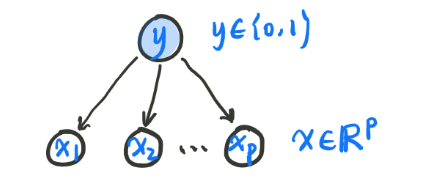
\includegraphics[width=.45\textwidth]{微信图片_20191104091918.png}
    \caption{条件独立性假设}
    \label{fig:my_label_1}
\end{figure}
\noindent 我们可以将其定义为$x_i\perp x_j|y\ (i \neq j)$。根据贝叶斯公式可以得:
\begin{equation}
    p(y|x)=\frac{p(x|y)p(y)}{p(x)}=\frac{p(x,y)}{p(x)}\propto p(x,y)
\end{equation}

而做条件独立性假设的最终目的,是为了简化运算。因为对于一个数据序列$x=(x_1,x_2,\cdots,x_p)$。如果$x_i$和$x_j$之间有关系的话,这个计算难度可能会变得很难,所以就假设各个变量之间是相互独立的。但是为了简化计算,这个假设太强了,显然有点不合理,没有充分利用数据之间的分布。

而我们将$y(0/1\rightarrow \mathrm{Seq})$就得到了Hidden Markov Model (HMM),这是我们得到HMM的第一种思路。

~\\
\noindent \textbf{高斯混合模型(Gaussian Mixture Model):}
高斯混合模型的概率图可以被我们描述为如下形式:
\begin{figure}[H]
    \centering
    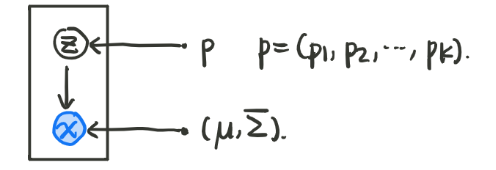
\includegraphics[width=.45\textwidth]{微信图片_20191223234640.png}
    \caption{GMM的概率图表达形式}
    \label{fig:my_label_1}
\end{figure}
我们根据一个离散的随机变量$Z$来选择是选取那个高斯分布,利用这个高斯分布$\mathcal{N}(\mu,\Sigma)$来采样得到我们想要的样本点。而且,离散随机变量$Z$符合一个离散分布$p = (p_1,p_2,\cdots,p_k)$。也就是$P(X|Z)\sim \mathcal{N}(\mu,\Sigma)$,而在此基础上加上时间的影响就构成了Hidden Markov Model,这是HMM的第二种引出方式。

~\\
\textbf{隐马尔可夫模型(Hidden Markov Model):}这个在我们之间的章节中有非常详细的描述,这里不再做过多的阐述,有兴趣的同学可以去仔细的观看。HMM中有两条非常重要的假设,齐次马尔可夫假设和观测独立假设,我们的计算基本都是基于这两个假设来的。

Hidden Markov Model的概率图模型如下所示:
\begin{figure}[H]
    \centering
    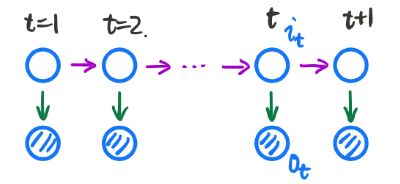
\includegraphics[width=.45\textwidth]{微信图片_20200107213811.png}
    \caption{Hidden Markov Model拓扑结构图}
    \label{fig:my_label_1}
\end{figure}
其中,$x_1$为observe data,$y_1$为lactent data,模型整体描述为$\lambda = (\pi,\mathcal{A},\mathcal{B})$。而实际上,我们还是感觉两个假设不太合理,限制了对数据集的利用,只是因为需要简化计算,所有没办法。但是,后来研究人员还是想消除假设,从而释放数据中更多的信息。

~\\
\textbf{最大熵马尔可夫模型(Maximum Entropy Markov Model):}
这里我们只对MEMM模型做一些简单的描述,尽量上直观的去解释。

MEMM是最大熵模型和HMM的结合体,它是一个判别模型。这里强调一下,它和HMM的主要区别是:\textbf{打破了HMM的观测独立假设。}这里我们后面会详细的描述。MEMM在建模过程中用到了公式(2)中,最大熵模型的求解结果,主体还是用的HMM的结构,所以,被称为最大熵马尔可夫模型。

MEMM的做法就是把输入分成两部分,1. 是所有的的$x_{1:T}$对$y$的输;2. 单独一个上一个状态$x_{t-1}$,local输入。有的同学可能会觉得有点奇怪,$x_{1:T}$中不就包括了$x_{t-1}$,对的实际上很多时候都只看$x_{1:T}$,这样分开说是为了便于理解在HMM上的改进。MEMM的概率图模型如下所示:
\begin{figure}[H]
    \centering
    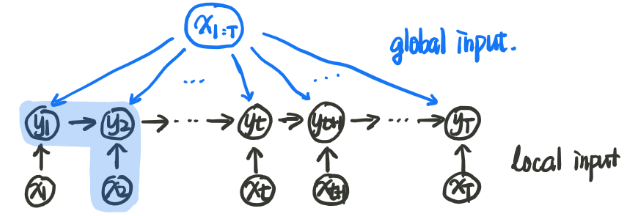
\includegraphics[width=.65\textwidth]{微信图片_20200221182717.png}
    \caption{MEMM的概率图模型}
    \label{fig:my_label_1}
\end{figure}

这小节的主要目的是引出我们为什么得到了Conditional Random Field。MEMM的细节不做过多解释。MEMM的诞生1. 首先将HMM中的观测独立假设给丢掉了,这样可以更多的使用原始数据中的信息;2. 而且,我们关注的问题从求解联合概率分布$P(X,Y)$转换成了求解$P(Y|X)$。在标注问题中并不需要计算那么多,求解$P(Y|X)$就够了。

~\\
\noindent \textbf{条件随机场(Conditional Random Field)}
虽然,MEMM有了很大的改进,但是在历史的舞台了,MEMM并没有大放光彩,这是为什么呢?由于MEMM有一个致命的问题叫做“Label Bias Problem”,这个问题主要产生的原因是局部归一化,这个问题还挺难的,这里简要的介绍一下,有兴趣的同学去看John Latterfy的相关文献。

我们简单介绍一下,看到图四中的阴影部分:为$P(y_2|y_1,x_2)$局部是一个条件概率。为了让最后的结果都是一个概率分布,我们必须要做归一化处理:
$$
\frac{\phi(y_1,x_1,y_2)}{\sum \phi (y_1,\cdots)}
$$
这就是局部归一化的意思,至于会出现怎样的原因,这里没说,后面再做出详细的分析。这个原因是因为有向图的原因造成的,那么我们吧有向图变成无向图不就可以解决这个问题了,于是条件随机场算法就诞生了。

\subsection{小结}
本小节我们从机器学习的整个框架中讨论了条件随机场是怎么来的,希望对同学们有一定的启发。判别模型和生成模型的概念还是挺重要的,搞懂之后,理解很多算法你会有不一样的感受。























\end{document}
